\subsection{\ga Variant Analysis}
\label{sec:resMutation}

In order to understand the DSE contributions of individual \ga aspects, we analyze the variants with respect to throughput achievement and exploration time of the synthetic domain, see \figref{fig:dse:tr}.

%Graph show the GA+LS(Hybrid) is the best.
\begin{figure}[h]
	\centering
	%\vspace{-10pt}
	\subfloat[Throughput Achievement]{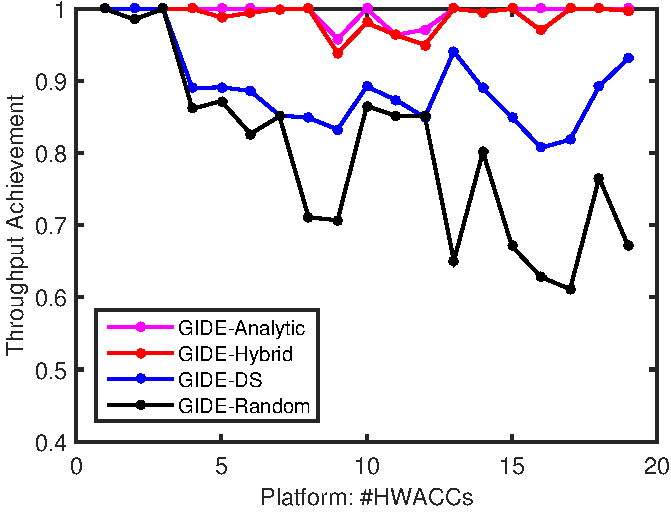
\includegraphics[width=.48\linewidth]{fig/prPAGASyn.pdf}\label{fig:paGASyn}}
	\hfill
	\subfloat[Exploration Time]{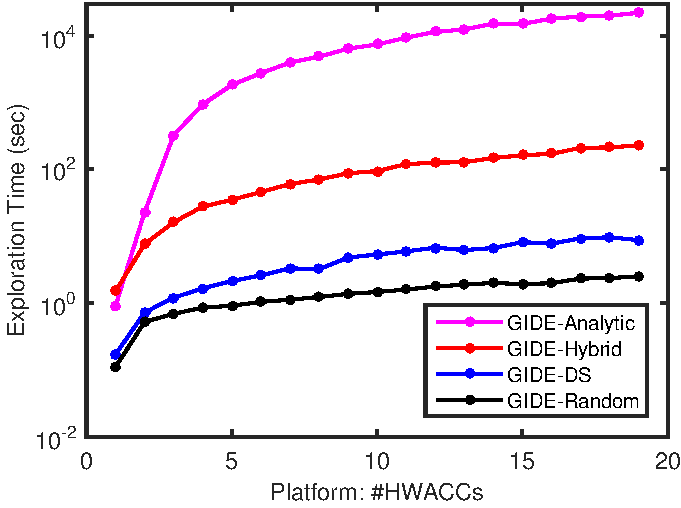
\includegraphics[width=.48\linewidth]{fig/prTimeGASyn.pdf}\label{fig:timeGASyn}}
	%\vspace{-5pt}
	\caption{Comparing \ga Variants (Synthetic)}
	\label{fig:dse:tr}
	%\vspace{-10pt}
\end{figure}




\gah and \gaana exhibit very similar achievements, see Fig.~\ref{fig:paGASyn}. They are close to optimal which is 99.41\% and 98.84\%, respectively, increasing the confidence in selecting the hybrid approach. Conversely, \gads is hampered with the DS accuracy in the guided local, only achieving 89.20\%. The inaccuracy of DS can lead to getting the local search being stuck at an invalid local optimum. \garand has the lowest achievement with 79.90\% on average over budget.

Looking at exploration time, \figref{fig:timeGASyn}, \garand is the fastest with 2 seconds. \gads, \gah and \gaana are around 5x, 100x, 10000x slower than random mutation. 
%
Comparing both achievement and exploration time sets out \gah as the best choice being 100x faster than \gaana while still achieving close to optimum results. Its two step of initial pruning with DS followed by more detailed Analytic Evaluation (AE) clearly sets it apart.  


\begingroup
\setlength{\columnsep}{8pt}%

\begin{wrapfigure}{l}{0.5\linewidth}
	%\vspace{-6pt}
	\begin{center}
		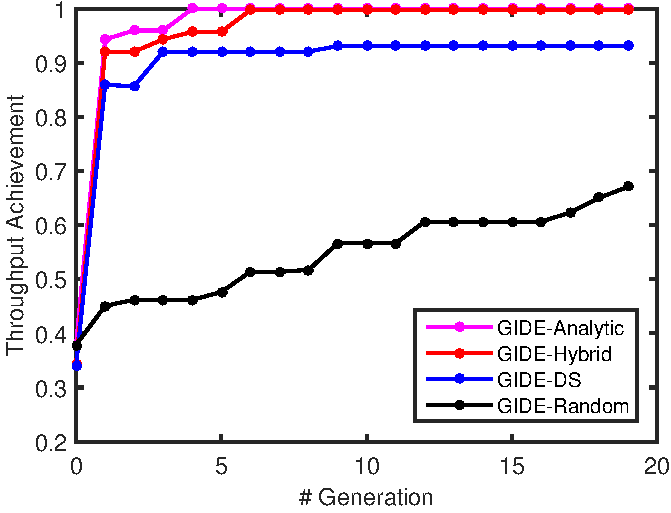
\includegraphics[width=\linewidth]{fig/prPAGenSyn.pdf}
	\end{center}
	%\vspace{-8pt}
	\caption{Improvement per Generation}
	\label{fig:paGenSyn}
	%\vspace{-4pt}
\end{wrapfigure}


To gain more insight with exploration generations, \figref{fig:paGenSyn} explores the achievement for a constant budget of $N$=19 in the synthetic domain. \gaana is the fastest to reach the best solution in only 5 generations. \gah is only 2 generations behind. \gads although rapidly reaching 90\% in a few generations, it cannot improve much over the remaining generations as it is stuck in an inaccurate local maximum. \garand needs many more generations, but steadily improves over them. 

\endgroup
%\begin{figure}[h]
%	\centering
%		\subfloat[OpenVX Domain]{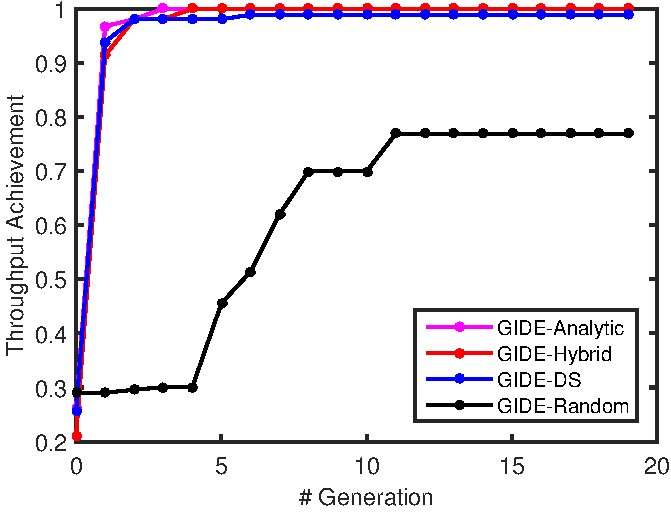
\includegraphics[width=.5\linewidth]{fig/prPAGenOpenVX.pdf}\label{fig:paGenOpenVX}}
%		\hfill
%		\subfloat[Synthetic Domain]{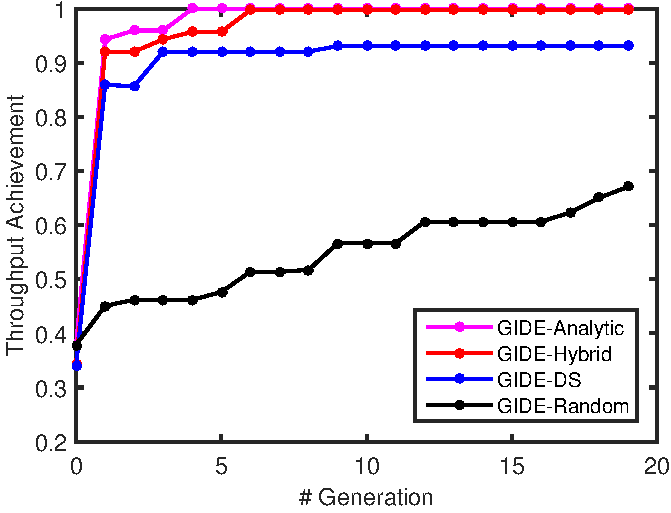
\includegraphics[width=.5\linewidth]{fig/prPAGenSyn.pdf}\label{fig:paGenSyn}}
%	\caption{Improvement per Generation}
%\end{figure}

%\begin{figure}[h]
%	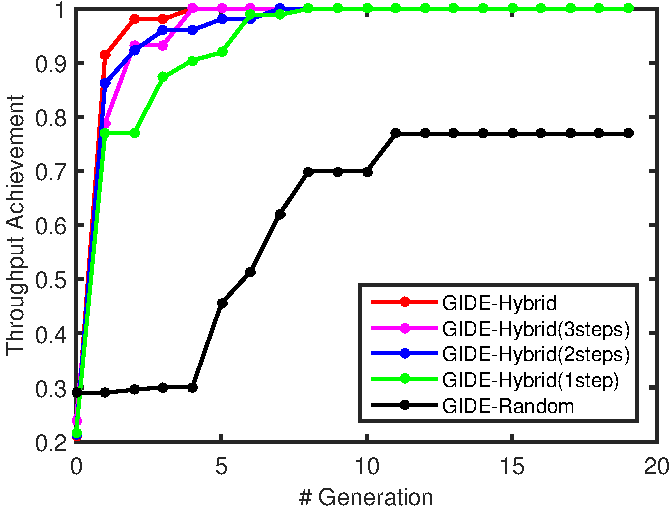
\includegraphics[width=.75\linewidth]{fig/prStepLimit.pdf}
%	\caption{OpenVX: GA limit number steps of local search}
%	\label{fig:stepLimit}
%\end{figure}



Our measurements demonstrate that the guided local search is highly efficient. To gain even further insight we measure
the average number of search steps and the effect of artificially limiting the search depth when exploring the OpenVX domain.
%Graph to show the step number of local search is acceptable. (Graph is need to re-draw)
\begin{figure}[h]
	\centering
		\subfloat[Average \# of Steps]{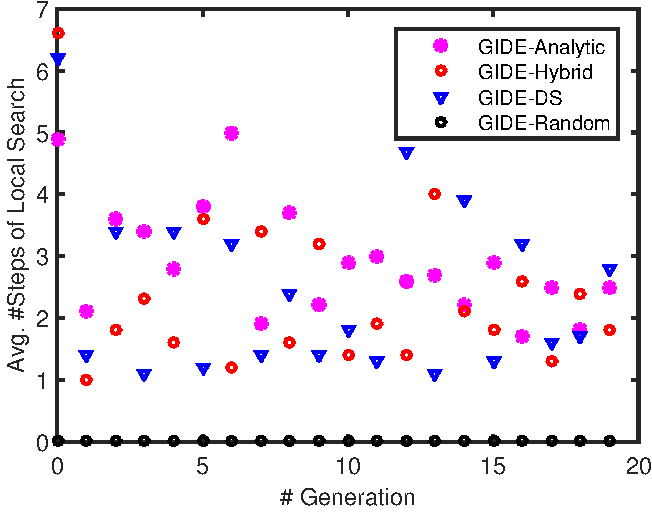
\includegraphics[width=.48\linewidth]{fig/prStepAve.pdf}\label{fig:stepAve}}
		\hfill
		\subfloat[Limit Steps of Local Search]{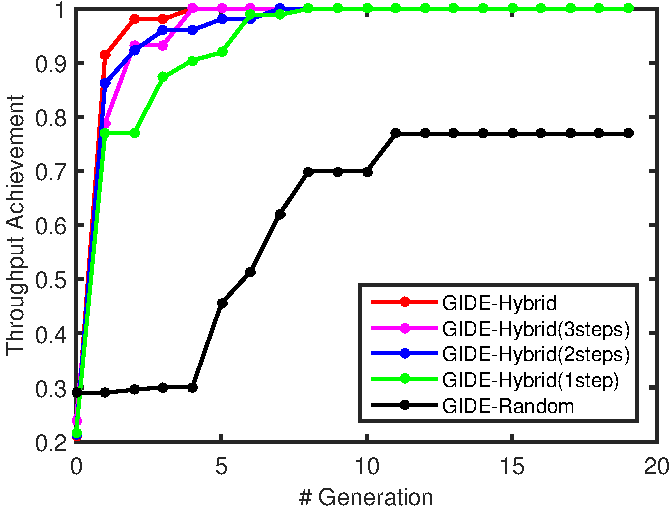
\includegraphics[width=.48\linewidth]{fig/prStepLimit.pdf}\label{fig:stepLimit}}
	\caption{Local Search Steps}
	\label{fig:step}
\end{figure}


%\begingroup
%\setlength{\columnsep}{8pt}%

%\begin{wrapfigure}{l}{0.5\linewidth}
	%\vspace{-6pt}
%	\begin{center}
%		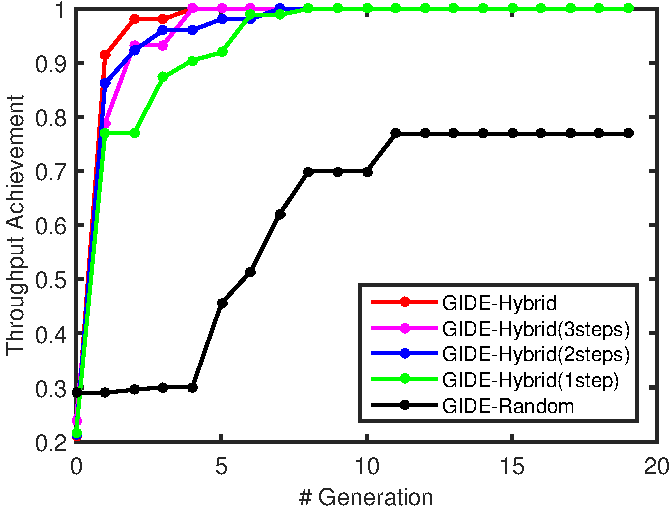
\includegraphics[width=\linewidth]{fig/prStepLimit.pdf}
%	\end{center}
	%\vspace{-8pt}
%	\caption{Limit Steps of Local Search}
%	\label{fig:stepLimit}
	%\vspace{-4pt}
%\end{wrapfigure}

\newtext{In} \figref{fig:stepAve}, \gaana, \gah and \gads have all a very low number of average steps across generations with, 2.91, 2.37, and 2.41 respectively. Even its maximum is low with 10 (\gaana), and 8 (for both \gah and \gads). The low number of steps can be explained with the exhaustive search of the neighborhood. Sparser sampling approaches, conversely, would need more steps. Limiting the maximum number of search steps only minimally impacts search performance as shown in \figref{fig:stepLimit} for the OpenVX domain. Although limiting to 3 steps, \gah still finds the optimum in 4 steps in this example. Further limiting the number of steps translates into requiring more generations (+3 with 2 steps, +4 with 1 step) nonetheless the same solutions are still reached. Due to the speed of DS evaluation, we do not limit the number of steps. 

%\endgroup

%GA summary - GS CUT
% GA with different mutations Trade-off between throughput achievement and exploration time.
%Summarizing the detailed results confirms our selection of \gah as the most suitable approach providing both s
%Random and DSS have the fast exploration, but the performance is bad.
%The Analytical and Hybrid has the almost highest performance.
%Hybrid is 100x faster than analytical evaluation.
%GA-Hybrid is the best choice for domain DSE for most cases.
%However, if want to get the highest performance design, and do not care about the exploring time, the GA-analytical could be considered.